\documentclass{article}

\usepackage[scale=0.75,top=2cm]{geometry}
\usepackage{tabularx}
\usepackage{algpseudocode}
\usepackage{multicol}
\usepackage{caption}
\usepackage{tikz}
\usepackage[utf8]{inputenc}
\usepackage{longtable}
\usepackage{array}
\usetikzlibrary{shapes}



\begin{document}
%----------------------------------------------------------------------------------------------------------------------------------------
\title{Project Report}
\author{Akshat Bisht 40053762}
\date{\today}
\maketitle
%----------------------------------------------------------------------------------------------------------------------------------------

\newpage
%----------------------------------------------------------------------------------------------------------------------------------------


\section{Introduction}
Brief description of the problem, its significance, the main message of the paper, and briefly mention the key results.

\section{Background} 
Contains some history about online coloring problem. Historical notes and references at the end of Chapter 5 can be helpful 
for this, but you should go beyond what's just written there.

\newpage

\section{New Algorithm}

This is where you describe your algorithm that you propose that is different from FirstFit and CBIP. You will evaluate this 
algorithm alongside FirstFit and CBIP.
\bigbreak
The Algorithm that we have implemented for this project isn't a greedy based algorithm, thus it is different from FirstFit. The algorithm's
computation procedure is similar to the CBIP algorithm except that at the end it uses \textbf{randomization}.\\
The Psuedocode for the is Algorithm is presented below.
		
	\begin{multicols}{2}% 2-column layout
	  \begin{minipage}{0.45\textwidth}
	    \begin{algorithmic}[1]% Taken from the algorithmicx package documentation
	      \Procedure{MyAlgorithm}{$G,\sigma$}
	      \State Initialize List L.
	      \State Compute $C_v \mbox{ - connected component of } v$
	      \State Compute bipartition of $C_v = S_v \cup \widetilde{S_v}$
	      \State \ \ \ \  v $\in S_v$ and $N(v) \subseteq \widetilde{S_v}$
	      \State L= colors \textbf{not} in $\widetilde{S_v} \mbox{ but present in } S_v$
	      \State Let \textit{i} be a color Randomly selected out of L.
	      \State Color \textit{v} with \textit{i}
	      \EndProcedure
	    \end{algorithmic}
	  \end{minipage}
	The Breadth First Search Algorithm is used to separate all the vertices that are in the $S_v$ and $\widetilde{S_v}$ . A set of all the vertices/colors that are not in $\widetilde {S_v}$ but are in $S_v$ is created. A color is selected from the set and assigned to the vertex.\\

	 In CBIP, we select color with the minimum color value from the set. But in our algorithm, the color is selected randomly from the set.

	\end{multicols}	


\section{Implementation Details}

\bigbreak
The implementation details of the code can be broken down into the following sections.\\

\textbf{Graph Representation:}\\

The graphs that can be successfully read by the program, should be in the same format as mentioned in the project.pdf (i.e MMC format). 
The code uses and adjacency matrix of boolean type to read the graphs that are inputted. The cells in the matrix are set to true if an edge exists
between the nodes. The use of an adjacency matrix helps making sure that the graphs that are being read are automatically converted to Bipartite 
Graphs(i.e \textit{Duplicating method}). A disadvantage of this method is that a lot of memory is wasted and this method may not be optimal for larger graphs or for machines with low memory.\\


\textbf{Important Methods and Variables :}\\

\textit{ReadNetworkRepoGraphs() }: Reads all the graphs downloaded from the Network Repository website.The extension of the files are
 "NetworkRepoGraph1.txt", "NetworkRepoGraph2.txt"... You can change the number of graphs to read to check the result by running the inner
 loop once instead of 5 times. If it is changed to 1 , then it will read only "NetworkRepoGraph1.txt" and you can check the results of 1 graph with 
the lowest number of nodes more carefully. \\ 

 \textit{ReadRandomGraphs() }: Reads all the graphs downloaded from the Random Graphs created by the class "RandomGraphs.java".The
 extension of the files are"RandomGraph1.txt", "RandomGraph2.txt"... You can change the number of graphs to read to check the result by 
running the inner loop once instead of 5 times. If it is changed to 1 , then it will read only "NetworkRepoGraph1.txt" and you can check the
 results of 1 graph with the lowest number of nodes more carefully.\\

\textit{createGraph()}:In the class "RandomGraphs.java", the createGraph() method, has an array with different integer values (number of nodes).
 An adjacency matrix is created and as we iterate through the 2D-boolean array. Initailly all values are False(no edge exist between nodes)
 by default. There is an in-built Java random function that produces integer values in the interval [1,11]. While being on a cell if the randomizer spits out an even number, the cell value is turned True (edge exists). Thus, $P(edge)= \frac{2}{5}$ and $P(\widetilde{edge})=\frac{3}{5}$.\\ 

\textit{RandomOrderInput()}: It fills up an array with all integer values in the interval [1,numberOfVertices], and then all the values in the array are
randomly shuffled using the Java randomizer.\\

\textit{Data()}: Prints the average of the number of colors used by each algorithm for each graph by using respectively. A graphical representation 
of this data is shown in the Result section of this report.\\

\textit{Iterations}: This global variable can be changed, depending upon how many times the user want to run all 3 algorithms for all the inputted 
graphs and see what the average values of the number of colors used by all algorithms for all the graphs will be. We ran 100 iterations and the 
average values computed are in a table in the result section of this report.\\

\textbf{Challenges :}\\

The most challenging part of this project was the coding of CBIP algorithm. The algorithm took some time to understand properly, but thanks to the
 Professor Pankratov and his Teaching Assistant(Ali Mohammed) we were able to grasp the concept. Coding the Breadth-First-Search(BFS)  
and keeping alternating depth level vertices in different sets was the most challenging, algorithmically speaking. \\

Some other challenges we faced in this program were due to extensive use of arrays in our program, we had to be really careful as most of the errors
 came from ArrayIndexOutOfBoundsException because array indices start from 0 while the vertices in the graphs start from 1.\\

Initially the code was tested with small graphs containing 5 to 10 vertices, as computing solutions of these graphs by hand was feasible.These small
 graphs were created to try and get the most number of colors from the FirstFit and CBIP algorithms (Adversarial Input). These graphs
 are also submitted with code.\\ 

We cannot be completely sure that this program is bug free. The input graph formats and graph naming conventions have to be correct, for the 
code to function as intended. We may have missed some edge cases. But because of extensive testing we are confident that the
 algorithmic executions are correct. 

\section{Experimental Details}

\bigbreak
This program was coded in Java. The version of Java used was Java version 14.\\
The system where this code was written used the windows operating system, had 16 Gigabytes of RAM and with an i5 processing chip. \\
The code was written in the Eclipse IDE. \\


\newpage

\section{Results}
2.5 pages long\\
This is where you present your findings, time-series plots, tables and comment on what you see. You need to analyze how the
performance of CBIP compares to FirstFit and Your Algorithm, any patterns that you found, any general observations. The 
deeper and the more interesting observations the better your grade will be.

\begin{center}
 \begin{tabular}{||p{2cm} | p{2cm} | p{2cm} | p{2cm} ||} 
\hline
\multicolumn{4}{|c|}{Network Repository Graphs} \\

 \hline
\hline
 Nodes & \multicolumn{3}{|c|}{Colors} \\
\hline
  & FirstFit & CBIP & MyAlgorithm \\ [0.5ex] 
 \hline\hline
 66 & 4.91 & 17.5 & 17.53 \\ 
 \hline
 101 & 6.41 & 3.08 & 3.08 \\
 \hline
 144 & 9.41 & 32.49 & 32.49 \\
 \hline
 204 & 6.36 & 29.05 & 28.23 \\
 \hline
 219 & 6.23 & 22.81 & 23.61\\ [1ex] 
 \hline
\end{tabular}
\end{center}




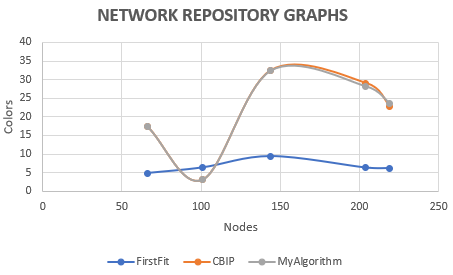
\includegraphics[width=0.75\textwidth]{NetworkRepoGraph}
\bigbreak
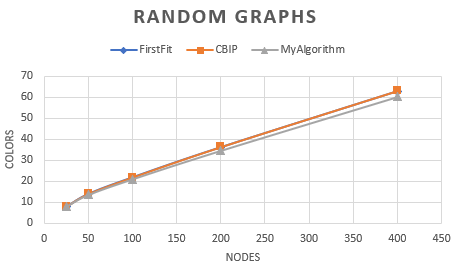
\includegraphics[width=0.75\textwidth]{RandomGraph}

\begin{center}
 \begin{tabular}{||p{2cm} | p{2cm} | p{2cm} | p{2cm} ||} 
\hline
\multicolumn{4}{|c|}{Random Graphs} \\
\hline
\hline
 Nodes & \multicolumn{3}{|c|}{Colors} \\
\hline
 & FirstFit & CBIP & MyAlgorithm \\ [0.5ex] 
 \hline\hline
 25 & 7.89 & 8.03 & 7.99 \\ 
 \hline
 50 & 14.02 & 14 & 13.58\\
 \hline
 100 & 21.94 & 21.93 & 21.04 \\
 \hline
 200 & 36.25 & 36.41 & 34.59 \\
 \hline
 400 & 62.88 & 63.19 & 60.16\\ [1ex] 
 \hline
\end{tabular}
\end{center}


\newpage

\section{Future Directions}
0.5 page\\
This is where you explain in which directionyou can extend this project. Mention interesting open problems, etc. If you had more time,
what thing would you have liked to try?
\newpage

\section{Bibliography}

%----------------------------------------------------------------------------------------------------------------------------------------



\newpage



\end{document}